\documentclass[conference]{IEEEtran}
% --- Paketler ---
\usepackage[utf8]{inputenc}
\usepackage[T1]{fontenc}
\usepackage[turkish]{babel}
\shorthandoff{=}          % babel-turkish '=' işaretini aktif yapar; tablolarda sorun çıkmasın
\usepackage{amsmath,amssymb}
\usepackage{graphicx}
\graphicspath{{figures/}{../figures/}} % Şekiller önce figures/ (Overleaf), bulunamazsa ../figures/ (yerel) altında aranır
\usepackage{booktabs}
\usepackage{tabularx}
\usepackage{array}
\usepackage{url}
\usepackage[hidelinks]{hyperref}
\usepackage{enumitem}

\newcolumntype{L}{>{\raggedright\arraybackslash}X}
\newcommand{\todo}[1]{\textcolor{red}{[#1]}}
\usepackage{xcolor}

\begin{document}

\title{ALL/AML Lösemi Alt Tip Sınıflandırması:\\ Literatür, Veri Setleri ve Keşifsel Veri Analizi\\ (Ara Rapor)}

\author{\IEEEauthorblockN{Mehmet Ali Erel}
\IEEEauthorblockA{Öğrenci No: 503020260086\\
Makine Öğrenmesi ve Anomali Tespiti\\
Video: \url{https://www.youtube.com/playlist?list=PLYyNtnt32IHs}\\
Kod: \url{https://github.com/malierel/all-aml-leukemia-classification}}}

\maketitle

\begin{abstract}
Akut lenfoblastik lösemi (ALL) ve akut miyeloid lösemi (AML) farklı tedavi protokolleri gerektiren iki lösemi alt tipidir; bu nedenle doğru ayrımları klinik açıdan kritiktir. Bu ara rapor, gen ifadesi mikrodizi verisinden ALL/AML alt tip sınıflandırması yapacak bir makine öğrenmesi çalışmasının temelini atmaktadır. Çalışmada Golub ve ark. (1999) verisi (72 örnek, 7.129 prob) ana veri seti, farklı nesil bir Affymetrix platformunda üretilmiş çok merkezli MILE çalışması (GEO GSE13159) ise dış doğrulama veri seti olarak belirlenmiştir. Golub verisini kullanan çalışmaların taranması, öznitelik seçiminin çoğu zaman çapraz doğrulama döngüsü dışında yapıldığını, nested CV kullanılmadığını ve sonuçların büyük ölçüde yalnızca doğruluk ile raporlandığını göstermiştir. Sızıntıyı düzelten çalışmalarda doğruluk \%92--95 düzeyine inerken sızıntılı tasarımlar \%100 bildirmektedir. EDA, Golub verisinde sınıf bilgisi kullanılmadan PCA'nın ALL ve AML'yi ayırdığını, eğitim setinde 602 genin FDR düzeltmesi sonrası anlamlı olduğunu ve bu genlerin \%86'sının bağımsız MILE verisinde de aynı yönde farklılaştığını göstermiştir; buna karşın iki platform arasındaki ölçek farkı, veri setine özgü normalizasyonu zorunlu kılmaktadır. Finalde sızıntısız nested CV ile en az üç yöntem karşılaştırılacak ve bulguların platformlar arası genellenebilirliği test edilecektir.
\end{abstract}

\begin{IEEEkeywords}
lösemi, ALL/AML sınıflandırması, mikrodizi, gen ifadesi, öznitelik seçimi, veri sızıntısı, nested çapraz doğrulama
\end{IEEEkeywords}

% =====================================================================
\section{Giriş}

\subsection{Problem ve Klinik Önem}
Akut lösemiler, kökenlerine göre lenfoid öncül hücrelerden gelişen ALL ve miyeloid öncül hücrelerden gelişen AML olarak iki ana gruba ayrılır~\cite{golub1999}. Bu ayrım klinik açıdan kritiktir: iki alt tip farklı kemoterapi rejimleriyle tedavi edilir ve yanlış sınıflandırma hem tedavi başarısını düşürür hem de gereksiz toksisiteye yol açar~\cite{golub1999}. Rutin tanı; morfoloji, immünofenotipleme ve sitogenetik gibi uzmanlık gerektiren birden fazla testin birlikte yorumlanmasına dayanır. Gen ifadesi profillemesi, bu ayrımı tek bir moleküler testle ve nesnel ölçütlerle yapma imkânı sunar~\cite{golub1999,haferlach2010}.

Bu çalışmada problem, \textbf{ALL ve AML alt tip sınıflandırması} olarak tanımlanmıştır. Ders modülündeki ``cancer / non-cancer'' ifadesi biyolojik olarak yanlıştır; her iki sınıf da lösemi alt tipidir.

\subsection{Mikrodizi Teknolojisi}
DNA mikrodizileri, binlerce genin mRNA düzeyini tek bir deneyde ölçen yonga tabanlı bir teknolojidir. Hastadan alınan örnekteki mRNA etiketlenir ve yonga üzerindeki bilinen dizilere sahip problarla hibridize edilir; her probdaki sinyal şiddeti ilgili genin ifade düzeyini yansıtır. Golub verisinde kullanılan Affymetrix Hu6800 yongası 7.129 prob içerir~\cite{golub1999}. Bu teknoloji örnek sayısından çok daha fazla öznitelik üretir ($p \gg n$). Bu durum aşırı öğrenme riskini artırır ve öznitelik seçimini zorunlu kılar~\cite{saeys2007}.

\subsection{Araştırma Soruları}
\begin{itemize}[leftmargin=*]
  \item \textbf{AS1:} Öznitelik seçimi çapraz doğrulama döngüsü içine alındığında (nested CV), Golub verisinde elde edilen performans literatürde sıkça bildirilen \%100 doğruluktan anlamlı ölçüde düşük müdür?
  \item \textbf{AS2:} Golub verisinde eğitilmiş modellerin performansı, farklı nesil bir platformda (HG-U133 Plus 2.0) üretilmiş bağımsız MILE verisine aktarıldığında korunur mu?
  \item \textbf{AS3:} Sınıf dengesizliği (\%65 ALL / \%35 AML) altında doğruluk ile dengeli doğruluk ve ROC-AUC arasında yöntemleri farklı sıralayacak kadar fark var mıdır?
\end{itemize}

\subsection{Katkılar}
\begin{itemize}[leftmargin=*]
  \item Golub verisi üzerindeki çalışmaların doğrulama protokollerini ve sızıntı risklerini karşılaştıran sistematik bir literatür özeti.
  \item Golub ve MILE verilerinin kalite, dağılım ve batch farkları açısından karşılaştırmalı keşifsel analizi (EDA).
  \item Finalde sızıntısız, tekrarlanabilir bir değerlendirme protokolü ve platformlar arası dış doğrulama için hazırlanmış bir kod deposu.
\end{itemize}

% =====================================================================
\section{Literatür Taraması}

\subsection{Arama Protokolü}
Tarama IEEE Xplore, PubMed ve Google Scholar üzerinde 1999--2026 aralığında yapılmıştır; son beş yıl (2021--2026) ayrıca taranmıştır. Kullanılan sorgular ve döndürdükleri sonuç sayıları Tablo~\ref{tab:sorgu}'de verilmiştir.

\begin{table}[htbp]
\caption{Arama sorguları ve sonuç sayıları}
\label{tab:sorgu}
\centering
\footnotesize
\begin{tabularx}{\columnwidth}{@{}c L c c@{}}
\toprule
\# & Sorgu & IEEE & Scholar \\
\midrule
1 & ``Golub'' AND leukemia AND (classification OR ``machine learning'') & \todo{} & \todo{} \\
2 & ``ALL'' AND ``AML'' AND ``gene expression'' AND (classifier OR ``feature selection'') & \todo{} & \todo{} \\
3 & microarray AND ``feature selection'' AND ``small sample'' AND cancer & \todo{} & \todo{} \\
4 & leukemia AND ``gene expression'' AND (``deep learning'' OR transformer) & \todo{} & \todo{} \\
5 & (``data leakage'' OR ``selection bias'') AND microarray AND ``cross-validation'' & \todo{} & \todo{} \\
\bottomrule
\end{tabularx}
\end{table}

\textbf{Dahil etme ölçütleri:} hakemli dergi veya konferans yayını; mikrodizi ya da RNA-seq ile lösemi veya kanser sınıflandırması; doğrulama yöntemi ve sayısal sonuç raporlanmış olması.
\textbf{Dışlama ölçütleri:} tam metnine erişilemeyen, doğrulama yöntemi belirtilmemiş, tekrar yayınlanmış veya DOI'si doğrulanamayan çalışmalar. Sonuçta 22 hakemli yayın ve bir ön baskı seçilmiştir; bunların 11'i son beş yıla aittir.

\subsection{Temel Çalışmalar ve Yöntem Ailesi}
Golub ve ark.~\cite{golub1999}, sinyal-gürültü oranıyla seçilen 50 gen ve ağırlıklı oylama yöntemiyle ALL/AML ayrımını yapmış; ayrıca sınıf bilgisi kullanılmadan kümelemenin bu iki sınıfı kendiliğinden ayırdığını göstermiştir. Sonraki çalışmalar bu veriyi bir kıyaslama standardına dönüştürmüştür. Furey ve ark.~\cite{furey2000} ve Guyon ve ark.~\cite{guyon2002} destek vektör makinelerini (SVM) öne çıkarmış; Guyon'un SVM-RFE yöntemi gömülü öznitelik seçiminin klasiği olmuştur. Dudoit ve ark.~\cite{dudoit2002} basit yöntemlerin (DLDA, k-NN) karmaşık yöntemlerden geri kalmadığını, Díaz-Uriarte ve Alvarez de Andrés~\cite{diaz2006} ise rastgele ormanların (RF) diğer yöntemlerle karşılaştırılabilir performans verdiğini göstermiştir. Saeys ve ark.~\cite{saeys2007} öznitelik seçimini filtre, sarmalayıcı ve gömülü yöntemler olarak sınıflandırmıştır.

\subsection{Doğrulama ve Veri Sızıntısı}
Ambroise ve McLachlan~\cite{ambroise2002}, genler tüm veri üzerinde seçildikten sonra yapılan çapraz doğrulamanın hatayı sistematik olarak düşük gösterdiğini (seçim yanlılığı) Golub verisi üzerinde göstermiştir. Düzeltilmiş dış 10-kat CV ile hata yaklaşık \%5 bulunmuştur. Varma ve Simon~\cite{varma2006}, hiperparametre seçimi de CV içinde yapıldığında yanlılığın sürdüğünü ve nested CV'nin gerçek hatayı neredeyse yansız tahmin ettiğini göstermiştir. Kapoor ve Narayanan~\cite{kapoor2023} ise veri sızıntısının günümüzde de 17 bilim alanında yaygın olduğunu raporlamıştır.

\subsection{Son Dönem Çalışmalar}
Son beş yılda metasezgisel ve hibrit öznitelik seçimi yöntemleri öne çıkmıştır~\cite{almazrua2022,elemam2022,osama2023,yaqoob2024}. Benzer yaklaşımlar Golub dışındaki lösemi verilerine de uygulanmıştır: Ilyas ve ark.~\cite{ilyas2023}, CuMiDa veritabanındaki GSE9476 verisinde 22.283 öznitelikten seçtikleri 25 genle doğrusal programlama tabanlı bir sınıflandırıcı kurmuş ve \%98,44 doğruluk bildirmiştir. Derin öğrenme tabanlı yaklaşımlar da önerilmiştir~\cite{alharbi2023,mallick2023}. Ancak tablo verisinde ağaç tabanlı modellerin derin modellerden çoğu zaman üstün olduğu bilinmektedir~\cite{grinsztajn2022}. Tablo verisi için transformer tabanlı bir temel model olan TabPFN~\cite{hollmann2025} küçük örneklemde güçlüdür ama yaklaşık 500 öznitelik sınırı nedeniyle gen ifadesi verisinde önce öznitelik seçimi gerektirir~\cite{zhou2025}. GenePT~\cite{chen2024} ise gen açıklamalarının LLM gömmelerini kullanan alternatif bir temsil sunmaktadır.

\subsection{Literatür Özet Tablosu}
Golub verisini kullanan çalışmaların özeti Tablo~\ref{tab:lit}'de verilmiştir.

\begin{table*}[t]
\caption{Golub verisini kullanan çalışmaların karşılaştırmalı özeti}
\label{tab:lit}
\centering
\footnotesize
\begin{tabularx}{\textwidth}{@{}l L l l l L L@{}}
\toprule
Yazar/Yıl & Ön işleme / öznitelik seçimi & Yöntem & Doğrulama & Seçim CV içinde mi? & En iyi sonuç & Not \\
\midrule
Golub 1999~\cite{golub1999} & SNR, 50 gen & Ağırlıklı oylama & LOOCV + 38/34 test & İçinde & 34 testin 29'unda kesin tahmin, tamamı doğru & 5 örnek belirsiz \\
Guyon 2002~\cite{guyon2002} & Standardizasyon; SVM-RFE, 2--16 gen & Doğrusal SVM & LOOCV + test & Dışında & 8--16 genle test hatası 0 & Seçim yanlılığı riski \\
Ambroise 2002~\cite{ambroise2002} & SVM-RFE, SFS & SVM, FLD & Dış 10-kat CV, .632+ & İçinde & $\sim$\%5 hata & Yanlılık düzeltmesi \\
Dudoit 2002~\cite{dudoit2002} & Kırpma 100--16.000, log$_{10}$; BW, 40 gen & DLDA, k-NN, CART vb. & 2:1 bölme $\times$200 & İçinde & Medyan 1 test hatası & Basit yöntemler yeterli \\
Díaz-Uriarte 2006~\cite{diaz2006} & Filtre yok; RF önem skoru, 2 gen & RF & .632+ bootstrap & İçinde & .632+ hata 0,075 & Gen listesi kararsız \\
Elemam 2022~\cite{elemam2022} & $\chi^2$, F, MI + SFS, 5 gen & SVM, KNN, DT, RF & 10-kat CV & Kısmen dışında & \%100 & Yalnızca doğruluk \\
Mallick 2023~\cite{mallick2023} & Seçim yok & 5 katmanlı DNN & 80/20 sabit bölme & Uygulanamaz & \%98,2--100 & $\sim$15 test örneği \\
Yaqoob 2024~\cite{yaqoob2024} & RDO, 4--14 gen & XGBoost & 3-kat CV, LOOCV & Dışında & \%99,87--100 & Örnek sayısında iç tutarsızlık \\
\bottomrule
\end{tabularx}
\end{table*}

\subsection{Literatürdeki Boşluk}
Golub verisinde yayımlanmış sonuçların çoğu \%95--100 doğruluk bildirmektedir. İncelenen sekiz çalışmanın hiçbiri nested CV kullanmamış, en az üçünde öznitelik seçimi kısmen ya da tamamen CV dışında yapılmıştır. Sınıflar dengesiz olduğu halde çoğu çalışma yalnızca doğruluk raporlamıştır. Sızıntıyı düzelten çalışmalarda~\cite{ambroise2002,diaz2006} hata \%5--7,5 düzeyine çıkmaktadır. Ayrıca hiçbir çalışma bulguları farklı bir platformda üretilmiş bağımsız bir veri setinde test etmemiştir; Golub'un test seti de aynı yongadan gelmektedir. Bu çalışma, sızıntısız nested CV, dengesizliğe duyarlı metrikler ve platformlar arası dış doğrulama ile bu boşluğu hedeflemektedir.

% =====================================================================
\section{Veri Setleri}
Ana veri seti olarak Golub ve ark.~\cite{golub1999} lösemi verisi, dış doğrulama için ise MILE çalışmasının Aşama~I verisi (GEO GSE13159)~\cite{haferlach2010} seçilmiştir.

\subsection{Golub Verisi}
Veri, Kaggle üzerinde CC0 (kamu malı) lisansıyla yayımlanan sürümden alınmıştır. Kemik iliği ve periferik kan örneklerinden oluşan 72 hastalık bu set, Affymetrix Hu6800 yongası (7.129 prob, 6.817 insan geni) ile ölçülmüştür. Referans bölünme 38 eğitim (27 ALL, 11 AML) ve 34 bağımsız test (20 ALL, 14 AML) örneğidir. Her hasta sütununun yanında Affymetrix'in P/A/M (Present/Absent/Marginal) tespit çağrısı yer alır ve hasta sütunları dosyada numara sırasında değildir.

\subsection{MILE Verisi (GSE13159)}
Microarray Innovations in LEukemia (MILE) çalışması, üç kıtadaki 11 merkezde yürütülmüş çok merkezli bir programdır~\cite{haferlach2010}. Aşama~I verisi 2.096 hastadan oluşur ve 18 tanı sınıfı içerir. Örnekler Ficoll ile saflaştırılmış mononükleer hücrelerden HG-U133 Plus 2.0 yongasıyla ölçülmüştür. Ön aşamada merkezler arası tekrarlanabilirliğin yüksek olduğu gösterilmiştir~\cite{kohlmann2008}. Bu çalışmada yalnızca ALL (C1--C8 alt sınıfları, $n=750$) ve AML alt sınıfları kullanılacaktır.

\subsection{Veri Setlerinin Karşılaştırması}
İki veri seti Tablo~\ref{tab:veri}'de yan yana özetlenmiştir.

\begin{table}[htbp]
\caption{Veri setlerinin karşılaştırması}
\label{tab:veri}
\centering
\footnotesize
\begin{tabularx}{\columnwidth}{@{}l L L@{}}
\toprule
Özellik & Golub (1999) & MILE Aşama I \\
\midrule
Erişim & Kaggle & GEO GSE13159 \\
Lisans & CC0 & GEO kamuya açık, atıf zorunlu \\
Merkez & Tek merkez & 3 kıtada 11 merkez \\
Doku & Kemik iliği, periferik kan & Kemik iliği, periferik kan (Ficoll) \\
Platform & Hu6800 (GPL80) & HG-U133 Plus 2.0 (GPL570) \\
$p$ & 7.129 prob & 54.675 prob seti \\
$n$ & 72 (38 / 34) & ALL+AML: 1.292 \\
Sınıflar & ALL 47 / AML 25 & ALL 750 / AML 542 \\
Ölçek & Ham MAS sinyali, negatif değerler var & Quantile normalize, 0--1 ölçeğinde, log benzeri \\
\bottomrule
\end{tabularx}
\end{table}

\subsection{Seçim Gerekçesi ve Uyumluluk}
MILE dört nedenle seçilmiştir. Birincisi, aynı klinik problemi (ALL/AML) içerir ve ALL grubu Golub'daki gibi hem B hem T soy ALL örneklerini kapsar. İkincisi, aynı üreticinin farklı nesil yongasıyla ölçüldüğü için platformlar arası genellenebilirliği test etmeye uygundur. Üçüncüsü, çok merkezli tasarımı gerçekçi bir batch etkisi içerir. Dördüncüsü, büyük örneklemi Golub'un $p \gg n$ rejiminin tersini sunar.

Uyumlaştırma için iki platformun prob kimlikleri GPL80 ve GPL570 anotasyonlarıyla gen sembollerine eşlenmiştir. Sembolü olmayan ve birden fazla gene eşlenen problar atılmış, aynı gene düşen problardan ortalama ifadesi en yüksek olan seçilmiştir; bu işlemden sonra iki platformda 4.975 ortak gen kalmıştır. Golub verisine kırpma (20--16.000) ve log$_2$ dönüşümü uygulanacaktır. MILE verisi ise GEO'da quantile normalize edilmiş ve 0--1 aralığına ölçeklenmiş olarak yayımlandığından bu dönüşüm ona uygulanmayacak; iki veri seti ortak genler üzerinde, her biri kendi içinde ölçeklenerek karşılaştırılacaktır. Sınıf oranlarının farklı olması ve MILE'daki alt tip heterojenliği yorumlarda dikkate alınacaktır.

% =====================================================================
\section{Keşifsel Veri Analizi (EDA)}
Bütün analizler Python ile yapılmış ve tek komutla (\texttt{python scripts/run\_eda.py}) yeniden üretilebilir. Golub test seti yalnızca betimleme ve batch karşılaştırması için kullanılmış; ayırt edici gen analizi yalnızca eğitim seti üzerinde yapılmıştır.

\subsection{Veri Kalitesi}
Golub etiketleri \texttt{actual.csv} dosyasından hasta numarasına göre eşlenmiş ve sınıf sayıları 27/11 (eğitim) ve 20/14 (test) olarak doğrulanmıştır. Test dosyasında hasta sütunları numara sırasında olmadığından, etiketler sütun sırasına göre atansaydı 34 test hastasının 14'ü yanlış etiketlenecekti. Veride eksik ya da sonsuz değer yoktur. Değerlerin \%28,67'si negatiftir (en küçük -28.400); negatif değerlerin \%99,28'i Affymetrix tarafından ``Absent'' olarak işaretlenmiştir, yani bu değerler arka plan çıkarımından kaynaklanan ölçüm gürültüsüdür. P/A/M çağrıları sınıf ve setler arasında benzerdir (``Present'' oranı \%25,6--\%29,7). 1.971 prob hiçbir hastada ``Present'' değildir; 58 AFFX kontrol probunun 34'ü de bu gruptadır.

MILE matrisinde 54.675 prob bulunmaktadır; bunların 45'i (tamamı AFFX kontrol probu) bütün hastalarda boştur ve çıkarıldıktan sonra eksik değer kalmamaktadır. Değerler 0--1 aralığındadır ve negatif değer yoktur. Her hastanın medyanı aynıdır (0,2496) ve sıralanmış hasta değerleri ortak sıralamadan en fazla 0,0057 sapmaktadır; bu, verinin quantile normalize edildiğini göstermektedir. Çarpıklık 0,70 ile Golub'un log$_2$ sonrası değerine yakındır, bir kez daha log alındığında ise -0,89 olmaktadır; bu nedenle MILE verisinin zaten log benzeri bir ölçekte olduğu ve kırpma ile log$_2$ dönüşümünün uygulanmaması gerektiği sonucuna varılmıştır. Seçilen ALL ve AML hastalarının 1.211'i kemik iliği, 81'i periferik kan örneğidir.
% \begin{figure}[t]
% \centering
% 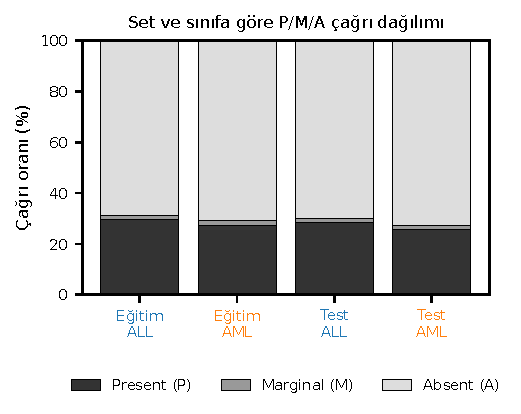
\includegraphics[width=\columnwidth]{fig02_pma_dagilimi.pdf}
% \caption{Set ve sınıfa göre P/M/A çağrı dağılımı.}
% \label{fig:pma}
% \end{figure}

\subsection{Betimsel İstatistikler ve Dönüşüm}
Sınıf dağılımı iki veri setinde de dengesizdir: Golub'da 47 ALL ve 25 AML (\%65,3 ALL), MILE'da 750 ALL ve 542 AML (\%58,0 ALL) bulunmaktadır. Golub test setinde AML oranı eğitim setinden yüksektir (\%28,9 ve \%41,2). MILE'da AML grubunun 351'i tek bir alt sınıfa (normal karyotip ve diğer anomaliler) aittir.

Ham ifade değerleri aşırı sağa çarpıktır (çarpıklık 7,08). Dudoit ve ark.~\cite{dudoit2002} izlenerek değerler 20--16.000 aralığına kırpılmış ve log$_2$ dönüşümü uygulanmıştır; çarpıklık 0,55'e inmiştir (Şekil~\ref{fig:dagilim}). Değerlerin \%32,72'si alt sınıra kırpılmaktadır. Dönüşümden sonra da hastalar arasında ölçek farkı sürmektedir: hasta medyanları 6,09--7,65 aralığında, en uç iki hastanın ortalamaları arasında yaklaşık 2,03 kat fark vardır. ALL ve AML ortalamaları neredeyse aynı olduğundan (6,965 ve 6,985) bu fark teknik kaynaklıdır.
\begin{figure}[t]
\centering
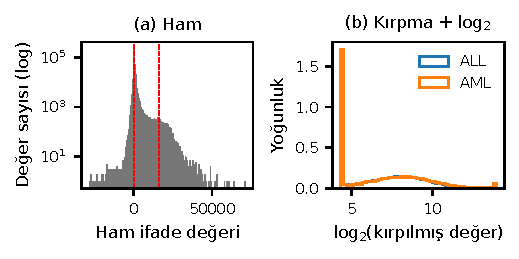
\includegraphics[width=\columnwidth]{fig03a_dagilim_ham_log.pdf}
\caption{(a) Ham ifade değerleri (kesikli çizgiler kırpma sınırları), (b) kırpma ve log$_2$ sonrası sınıf bazında dağılım.}
\label{fig:dagilim}
\end{figure}
% \begin{figure*}[t]
% \centering
% 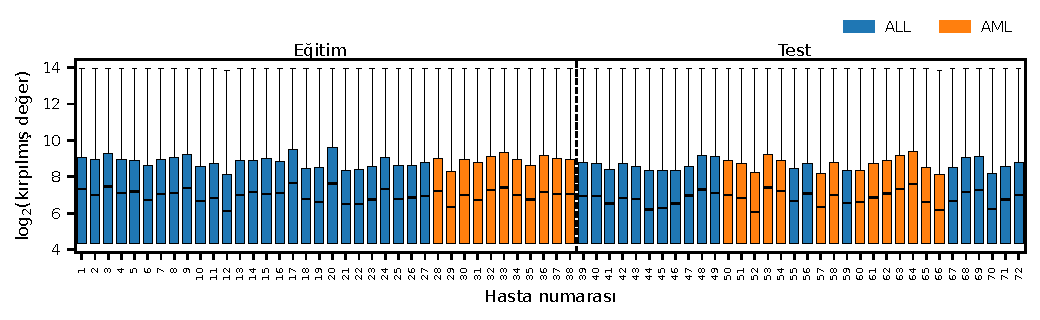
\includegraphics[width=\textwidth]{fig03b_ornek_kutu.pdf}
% \caption{Kırpma ve log$_2$ sonrası hasta bazında kutu grafiği.}
% \label{fig:kutu}
% \end{figure*}

\subsection{Boyut İndirgeme}
AFFX probları çıkarılmış 7.071 gen üzerinde yapılan PCA'da ilk iki bileşen varyansın \%17,67'sini açıklamaktadır; varyansın \%50'si için 13, \%90'ı için 54 bileşen gerekmektedir. Sınıf bilgisi kullanılmadığı halde PC1 ALL ve AML'yi ayırmaktadır (Mann--Whitney $1{,}8 \times 10^{-10}$; Şekil~\ref{fig:pca}), bu da Golub ve ark.~\cite{golub1999}'nin gözlemiyle uyumludur. Ancak ayrım kısmidir: sınıf siluet skoru PCA, t-SNE ve UMAP'te 0,27--0,30 aralığındadır. Eğitim ve test hastaları büyük ölçüde iç içedir (set siluet skoru 0,04--0,05). t-SNE ve UMAP'te eğitim setindeki AML hastaları sıkı bir küme oluştururken test setindeki AML hastaları daha dağınıktır (Şekil~\ref{fig:tsne}); bu, test AML'lerinin daha heterojen olduğuna işaret etmektedir. MILE'da da ortak genler üzerinde yapılan PCA iki sınıfı ayırmakta, sınıf siluet skoru Golub'dakinden yüksektir (0,44 ve 0,29).
\begin{figure}[t]
\centering
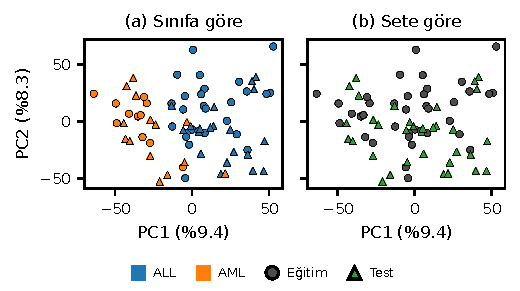
\includegraphics[width=\columnwidth]{fig04b_pca_pc1_pc2.pdf}
\caption{PC1--PC2 düzlemi: (a) sınıfa göre, (b) sete göre.}
\label{fig:pca}
\end{figure}
% \begin{figure}[t]
% \centering
% 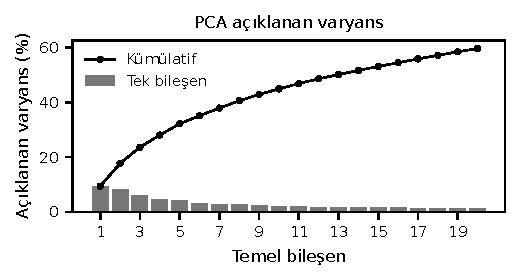
\includegraphics[width=\columnwidth]{fig04a_pca_varyans.pdf}
% \caption{PCA açıklanan varyans.}
% \label{fig:pcavar}
% \end{figure}
\begin{figure}[t]
\centering
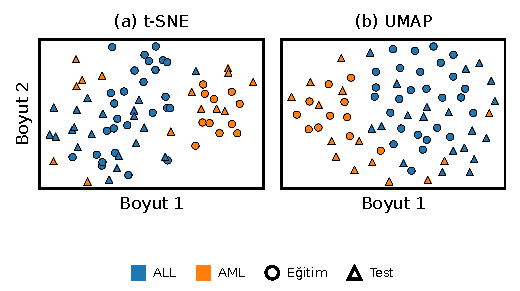
\includegraphics[width=\columnwidth]{fig04c_tsne_umap.pdf}
\caption{Golub verisinin (a) t-SNE ve (b) UMAP gömmeleri; daireler eğitim, üçgenler test hastaları.}
\label{fig:tsne}
\end{figure}

\subsection{Ayırt Edici Genler}
Yalnızca eğitim setinde (38 hasta), iki sınıfta da sabit olan 476 gen çıkarıldıktan sonra kalan 6.595 gene Welch t-testi ve Benjamini--Hochberg FDR düzeltmesi uygulanmıştır. 602 gen $q<0{,}05$ ile anlamlıdır (274'ü AML'de, 328'i ALL'de yüksek); bunların 410'u en az iki kat fark göstermektedir. En anlamlı 50 genle yapılan hiyerarşik kümeleme hastaları sınıflarıyla yüksek uyumla ayırmaktadır (düzeltilmiş Rand indeksi 0,79; Şekil~\ref{fig:isi}). Listenin başında CST3, Zyxin, CD33 (AML) ve CD19, TCF3 (ALL) gibi soy belirteçleri yer almaktadır. Bu genler tüm eğitim seti üzerinde seçildiğinden kümeleme sonucu iyimserdir; modellemede gen seçimi çapraz doğrulama katları içinde yapılacaktır~\cite{ambroise2002}.
\begin{figure}[t]
\centering
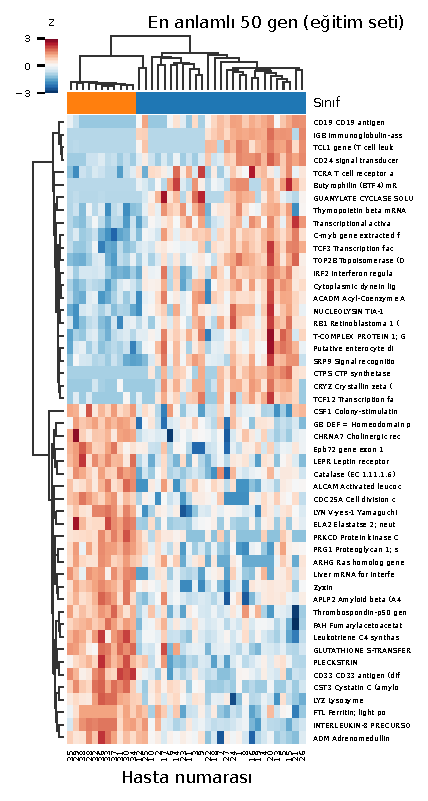
\includegraphics[width=\columnwidth]{fig05b_isi_haritasi_top50.pdf}
\caption{Eğitim setinde en anlamlı 50 genin z-skor ısı haritası ve hiyerarşik kümeleme.}
\label{fig:isi}
\end{figure}
% \begin{figure}[t]
% \centering
% 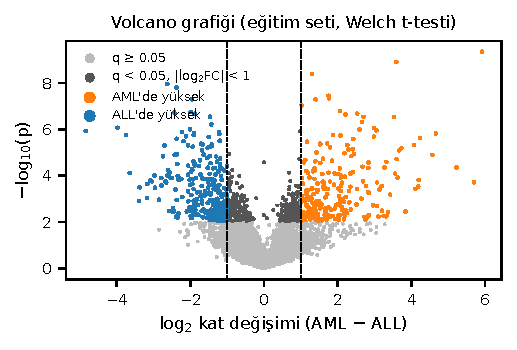
\includegraphics[width=\columnwidth]{fig05a_volcano.pdf}
% \caption{Volcano grafiği (eğitim seti).}
% \label{fig:volcano}
% \end{figure}

\subsection{Batch Analizi}
Test setinde AML oranı daha yüksek olduğundan (\%28,9 ve \%41,2) eğitim--test karşılaştırması yalnızca ALL hastaları arasında yapılmıştır. Test hastalarının genel ifade düzeyi her iki sınıfta da biraz daha düşüktür ve ALL hastalarının PCA'sında PC2 setleri ayırmaktadır (p = $4{,}3 \times 10^{-4}$). Gen bazında KS testinde 834 gen $p<0{,}05$ vermektedir (şans eseri beklenen 245), ancak FDR sonrası yalnızca 22 gen anlamlı kalmaktadır; her hasta kendi medyanına göre ortalandığında bu sayı 2'ye düşmektedir. Batch farkı zayıf, yaygın ve büyük ölçüde ölçek kaymasından kaynaklıdır.

Golub ve MILE ortak 4.975 gen üzerinde karşılaştırılmıştır. MILE 750 ALL ve 542 AML hastası içermekte ve quantile normalize edilmiş 0--1 ölçeğinde yayımlanmaktadır. Ham değerler doğrudan birleştirildiğinde PC1 varyansın \%97,2'sini açıklamakta ve yalnızca veri setini ayırmaktadır (veri seti siluet 0,99, sınıf siluet -0,00). Her gen kendi veri seti içinde z-skora çevrildiğinde veri seti farkı kaybolmakta, ALL/AML ayrımı ise iki veri setinde de aynı yönde ortaya çıkmaktadır (Şekil~\ref{fig:birlesik}). Golub eğitim setinde anlamlı bulunan genlerin \%86,0'ı MILE'da da aynı yönde farklıdır (tüm genlerde bu oran \%59,7); en anlamlı 50 genin 47'si tutarlıdır. Ters yönde çıkan genler (CDC25A, DYNLL1, UBE2V2) arasındaki CDC25A, Golub eğitim--test karşılaştırmasında da batch farkı gösteren tek ``en iyi 50'' genidir (Şekil~\ref{fig:yon}).
\begin{figure*}[t]
\centering
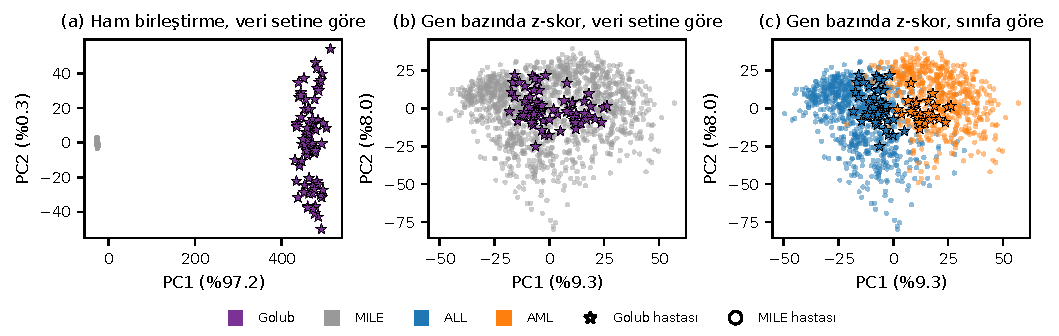
\includegraphics[width=\textwidth]{fig08b_birlesik_pca.pdf}
\caption{Golub ve MILE ortak genlerde birleşik PCA: (a) ham değerler, (b)--(c) gen bazında veri seti içi z-skor.}
\label{fig:birlesik}
\end{figure*}
\begin{figure}[t]
\centering
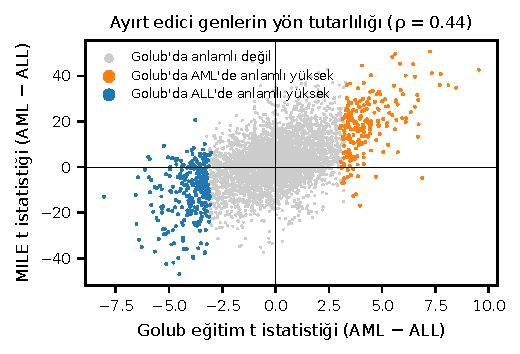
\includegraphics[width=\columnwidth]{fig08c_yon_tutarliligi.pdf}
\caption{Golub eğitim ve MILE t istatistikleri; renkli noktalar Golub'da anlamlı genler.}
\label{fig:yon}
\end{figure}
% \begin{figure}[t]
% \centering
% 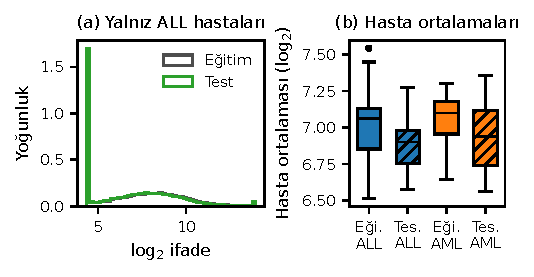
\includegraphics[width=\columnwidth]{fig06a_batch_dagilim.pdf}
% \caption{Golub eğitim--test karşılaştırması.}
% \label{fig:batch}
% \end{figure}
% \begin{figure}[t]
% \centering
% 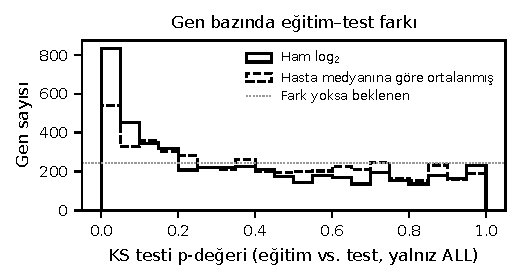
\includegraphics[width=\columnwidth]{fig06b_ks_pdegerleri.pdf}
% \caption{Gen bazında eğitim--test KS p-değerleri.}
% \label{fig:ks}
% \end{figure}
% \begin{figure}[t]
% \centering
% 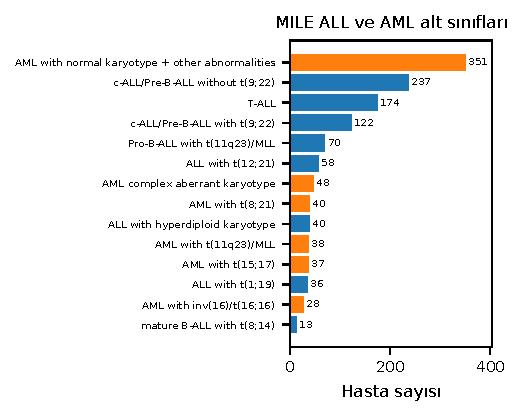
\includegraphics[width=\columnwidth]{fig07a_mile_alt_siniflar.pdf}
% \caption{MILE ALL ve AML alt sınıfları.}
% \label{fig:mile}
% \end{figure}
% \begin{figure}[t]
% \centering
% 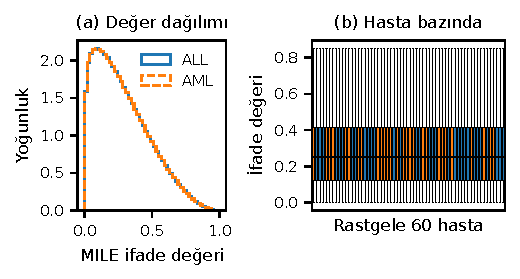
\includegraphics[width=\columnwidth]{fig07b_mile_olcek.pdf}
% \caption{MILE değer dağılımı ve hasta bazında kutu grafiği.}
% \label{fig:mileolcek}
% \end{figure}
% \begin{figure*}[t]
% \centering
% 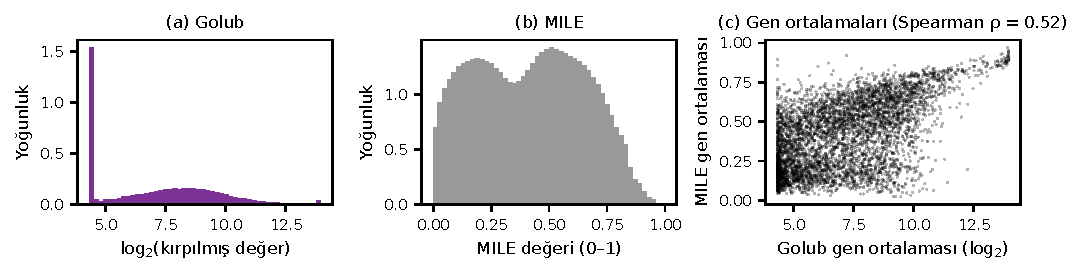
\includegraphics[width=\textwidth]{fig08a_golub_mile_olcek.pdf}
% \caption{Golub ve MILE ölçek karşılaştırması.}
% \label{fig:olcek}
% \end{figure*}

\subsection{Bulguların Özeti ve Modelleme İçin Çıkarımlar}
\begin{enumerate}[leftmargin=*]
  \item Golub etiketleri hasta numarasıyla eşlendi; sınıflar 27/11 (eğitim) ve 20/14 (test). Sütun sırasına göre eşleseydik testte 14 hasta yanlış etiketlenirdi. \textit{Çıkarım:} Etiketler her zaman hasta numarasıyla eşlenmeli; yükleyicideki assert kontrolleri korunmalı.
  \item Golub'da NaN/INF yok (0/0); değerlerin \%28,67'si negatif ve negatiflerin \%99,28'i 'Absent'. \textit{Çıkarım:} Modüldeki INF doldurma adımına bu veride gerek yok; negatifler ölçüm gürültüsü olduğu için alttan kırpılmalı.
  \item Ham değerler çok çarpık (çarpıklık 7,08); 20–16.000 kırpma + log2 sonrası 0,55. Değerlerin \%32,72'si alt sınıra yığılıyor. \textit{Çıkarım:} Kırpma + log2 Golub için standart ön işleme olmalı; her değere ayrı uygulandığı için sızıntı yaratmaz.
  \item 1.971 prob hiçbir hastada 'Present' değil; 58 AFFX kontrol probunun 34'ü de öyle. \textit{Çıkarım:} AFFX probları atılmalı; düşük ifade/varyans filtresi uygulanmalı ama yalnızca CV eğitim katlarında öğrenilmeli.
  \item Hasta ortalamaları arasında yaklaşık 2,03 kat fark var (log2 sonrası medyanlar 6,09–7,65); bu fark sınıfla ilişkili değil. \textit{Çıkarım:} Hasta bazında normalizasyon (ör. medyana göre ortalama) pipeline'da ablasyonla denenmeli.
  \item PCA'da sınıf bilgisi verilmeden PC1 ALL ile AML'yi ayırıyor (p = 1.8e-10); ancak PC1+PC2 varyansın yalnızca \%17,67'sini açıklıyor ve sınıf siluet skoru 0,29–0,30. \textit{Çıkarım:} Sınıf sinyali güçlü ama tek yöne sığmıyor; öznitelik seçimi ya da çok bileşenli doğrusal modeller uygun.
  \item Yalnız eğitim setinde 602 gen BH-FDR q < 0,05 ile anlamlı (410'u en az 2 kat farklı); en iyi 50 genle kümeleme sınıflarla ARI = 0,79 uyumlu. \textit{Çıkarım:} Az genle iyi ayrım mümkün; ama gen seçimi nested CV'nin her katında ayrı yapılmalı (seçim yanlılığı).
  \item Sınıf oranları dengesiz: Golub'da \%65,3 ALL; test setinde AML oranı eğitimden yüksek (eğitimde \%28,9, testte \%41,2). \textit{Çıkarım:} Stratified bölme, class\_weight ve dengeli doğruluk/ROC-AUC gibi dengesizliğe duyarlı metrikler kullanılmalı.
  \item Golub eğitim–test arasında hafif ama yaygın batch farkı: yalnız ALL'de 834 gen KS p < 0,05 (beklenen 245), FDR ile 22; hasta medyanına göre ortalayınca 2'ye iniyor. \textit{Çıkarım:} Batch farkının çoğu ölçek kayması; hasta bazında normalizasyon bunu büyük ölçüde gideriyor.
  \item MILE'da 750 ALL ve 542 AML var; veri quantile normalize, 0–1 ölçeğinde ve log benzeri (çarpıklık 0,70). Ortak gen sayısı 4.975. \textit{Çıkarım:} MILE'a kırpma + log2 uygulanmamalı; iki veri seti ortak genler üzerinden, her biri kendi içinde ölçeklenerek kullanılmalı.
  \item Ham birleştirmede veri seti farkı her şeyi bastırıyor (veri seti siluet 0,99, sınıf -0,00); gen bazında z-skor sonrası sınıf siluet 0,35, veri seti -0,18. \textit{Çıkarım:} Golub'da eğitilen model MILE'a uygulanacaksa genler her veri setinde ayrı ölçeklenmeli.
  \item Golub eğitimde anlamlı genlerin \%86,0'ı MILE'da da aynı yönde farklı; en iyi 50 genin 47'si tutarlı. Ters çıkanlar: CDC25A, DYNLL1, UBE2V2. \textit{Çıkarım:} Golub'da seçilen genler platformlar arası büyük ölçüde geçerli (AS2 için olumlu işaret); tutarsız genler yorumlanabilirlik bölümünde tartışılmalı.
\end{enumerate}

% =====================================================================
\section{Finale Kadar Plan}
Finalde üç yöntem, aynı sızıntısız pipeline içinde (imputasyon $\rightarrow$ kırpma ve log$_2$ (yalnızca Golub; MILE zaten normalize) $\rightarrow$ varyans filtresi $\rightarrow$ öznitelik seçimi $\rightarrow$ ölçekleme $\rightarrow$ model) ve aynı nested CV katlarında karşılaştırılacaktır.

\subsection{Seçilmesi Planlanan Yöntemler}
Planlanan yöntemler Tablo~\ref{tab:yontem}'de verilmiştir. Modülde verilen karar ağacı, taban çizgisi olarak ayrıca raporlanacaktır.

\begin{table}[htbp]
\caption{Planlanan yöntemler}
\label{tab:yontem}
\centering
\footnotesize
\begin{tabularx}{\columnwidth}{@{}l L l@{}}
\toprule
Yöntem & Gerekçe & Hiperparametreler \\
\midrule
Elastic-Net LR & Doğrusal, yorumlanabilir; gömülü öznitelik seçimi; $p \gg n$ için güçlü taban çizgisi & $C$, l1\_ratio \\
SVM (doğrusal, RBF) & Golub literatüründe en yaygın yöntem~\cite{furey2000,guyon2002}; doğrudan karşılaştırma & $C$, $\gamma$ \\
Rastgele Orman & Doğrusal olmayan, ölçeklemeye duyarsız; öznitelik önem skoru~\cite{diaz2006} & n\_estimators, max\_features \\
\bottomrule
\end{tabularx}
\end{table}

\subsection{Hedeflenen Bonuslar}
\begin{itemize}[leftmargin=*]
  \item \textbf{B1 -- Derin öğrenme:} dropout ve weight decay'li MLP; aynı dış CV katlarıyla, en az 5 seed.
  \item \textbf{B2 -- Transformer:} TabPFN v2~\cite{hollmann2025}; 500 öznitelik sınırı nedeniyle iç katlarda öznitelik seçimiyle birlikte~\cite{zhou2025}.
  \item \textbf{B4 -- Üçüncü veri seti (opsiyonel):} Armstrong ve ark.~\cite{armstrong2002} verisi, süre kalırsa.
\end{itemize}

\subsection{Takvim}
\begin{table}[htbp]
\caption{Finale kadar takvim}
\centering
\footnotesize
\begin{tabularx}{\columnwidth}{@{}l L@{}}
\toprule
Hafta & İş \\
\midrule
Ara rapor & EDA, ara rapor ve ara video teslimi \\
+1 & Pipeline, nested CV altyapısı, sabit 38/34 bölme deneyleri \\
+2 & Üç yöntemle ana deneyler, hiperparametre arama, istatistiksel test \\
+3 & MILE'a aynı protokolün uygulanması \\
+4 & Bonus deneyleri (B1, B2) \\
+5 & Yorumlanabilirlik, ablasyon, IEEE raporu ve final videosu \\
\bottomrule
\end{tabularx}
\end{table}

\subsection{Riskler}
\begin{table}[htbp]
\caption{Riskler ve önlemler}
\centering
\footnotesize
\begin{tabularx}{\columnwidth}{@{}L L@{}}
\toprule
Risk & Önlem \\
\midrule
Golub--MILE ortak gen sayısının düşük çıkması & Gen sembolü düzeyinde eşleme; ortak genlerle sınırlı analiz \\
Platformlar arası batch etkisi & Her veri setinde ayrı nested CV; örnek içi standardizasyon denemesi \\
Küçük örneklemde yüksek varyans & Tekrarlı CV ($\geq$5 seed), güven aralıkları, eşleştirilmiş istatistiksel test \\
Derin modellerin aşırı öğrenmesi & Erken durdurma iç katlarda; sonuçların dürüstçe raporlanması~\cite{grinsztajn2022} \\
MILE'ın büyük boyutu & Varyans filtresiyle boyut azaltma, paralel CV \\
\bottomrule
\end{tabularx}
\end{table}

% =====================================================================
\section*{Teşekkür ve GenAI Beyanı}
Bu raporun hazırlanmasında Anthropic Claude Opus 5.5 ve Google NotebookLM araçlarından yararlanılmıştır. Ayrıntılı kullanım beyanı ekte sunulmuştur. \todo{Ek GenAI beyanına göre güncellenecek.}

% =====================================================================
\begin{thebibliography}{99}
\bibitem{golub1999} T. R. Golub \textit{et al.}, ``Molecular classification of cancer: Class discovery and class prediction by gene expression monitoring,'' \textit{Science}, vol. 286, no. 5439, pp. 531--537, 1999, doi: 10.1126/science.286.5439.531.
\bibitem{furey2000} T. S. Furey \textit{et al.}, ``Support vector machine classification and validation of cancer tissue samples using microarray expression data,'' \textit{Bioinformatics}, vol. 16, no. 10, pp. 906--914, 2000, doi: 10.1093/bioinformatics/16.10.906.
\bibitem{guyon2002} I. Guyon, J. Weston, S. Barnhill, and V. Vapnik, ``Gene selection for cancer classification using support vector machines,'' \textit{Mach. Learn.}, vol. 46, pp. 389--422, 2002, doi: 10.1023/A:1012487302797.
\bibitem{dudoit2002} S. Dudoit, J. Fridlyand, and T. P. Speed, ``Comparison of discrimination methods for the classification of tumors using gene expression data,'' \textit{J. Amer. Stat. Assoc.}, vol. 97, no. 457, pp. 77--87, 2002, doi: 10.1198/016214502753479248.
\bibitem{ambroise2002} C. Ambroise and G. J. McLachlan, ``Selection bias in gene extraction on the basis of microarray gene-expression data,'' \textit{Proc. Natl. Acad. Sci. USA}, vol. 99, no. 10, pp. 6562--6566, 2002, doi: 10.1073/pnas.102102699.
\bibitem{saeys2007} Y. Saeys, I. Inza, and P. Larrañaga, ``A review of feature selection techniques in bioinformatics,'' \textit{Bioinformatics}, vol. 23, no. 19, pp. 2507--2517, 2007, doi: 10.1093/bioinformatics/btm344.
\bibitem{diaz2006} R. Díaz-Uriarte and S. Alvarez de Andrés, ``Gene selection and classification of microarray data using random forest,'' \textit{BMC Bioinformatics}, vol. 7, art. 3, 2006, doi: 10.1186/1471-2105-7-3.
\bibitem{varma2006} S. Varma and R. Simon, ``Bias in error estimation when using cross-validation for model selection,'' \textit{BMC Bioinformatics}, vol. 7, art. 91, 2006, doi: 10.1186/1471-2105-7-91.
\bibitem{kapoor2023} S. Kapoor and A. Narayanan, ``Leakage and the reproducibility crisis in machine-learning-based science,'' \textit{Patterns}, vol. 4, no. 9, art. 100804, 2023, doi: 10.1016/j.patter.2023.100804.
\bibitem{haferlach2010} T. Haferlach \textit{et al.}, ``Clinical utility of microarray-based gene expression profiling in the diagnosis and subclassification of leukemia: Report from the International Microarray Innovations in Leukemia Study Group,'' \textit{J. Clin. Oncol.}, vol. 28, no. 15, pp. 2529--2537, 2010, doi: 10.1200/JCO.2009.23.4732.
\bibitem{kohlmann2008} A. Kohlmann \textit{et al.}, ``An international standardization programme towards the application of gene expression profiling in routine leukaemia diagnostics: The Microarray Innovations in LEukemia study prephase,'' \textit{Br. J. Haematol.}, vol. 142, no. 5, pp. 802--807, 2008, doi: 10.1111/j.1365-2141.2008.07261.x.
\bibitem{armstrong2002} S. A. Armstrong \textit{et al.}, ``MLL translocations specify a distinct gene expression profile that distinguishes a unique leukemia,'' \textit{Nat. Genet.}, vol. 30, no. 1, pp. 41--47, 2002, doi: 10.1038/ng765.
\bibitem{almazrua2022} H. AlMazrua and H. Alshamlan, ``A comprehensive survey of recent hybrid feature selection methods in cancer microarray gene expression data,'' \textit{IEEE Access}, vol. 10, pp. 71427--71449, 2022, doi: 10.1109/ACCESS.2022.3185226.
\bibitem{elemam2022} T. Elemam and M. Elshrkawey, ``A highly discriminative hybrid feature selection algorithm for cancer diagnosis,'' \textit{Sci. World J.}, vol. 2022, art. 1056490, 2022, doi: 10.1155/2022/1056490.
\bibitem{grinsztajn2022} L. Grinsztajn, E. Oyallon, and G. Varoquaux, ``Why do tree-based models still outperform deep learning on typical tabular data?,'' in \textit{Proc. NeurIPS}, 2022, doi: 10.48550/arXiv.2207.08815.
\bibitem{osama2023} S. Osama, H. Shaban, and A. A. Ali, ``Gene reduction and machine learning algorithms for cancer classification based on microarray gene expression data: A comprehensive review,'' \textit{Expert Syst. Appl.}, vol. 213, art. 118946, 2023, doi: 10.1016/j.eswa.2022.118946.
\bibitem{alharbi2023} F. Alharbi and A. Vakanski, ``Machine learning methods for cancer classification using gene expression data: A review,'' \textit{Bioengineering}, vol. 10, no. 2, art. 173, 2023, doi: 10.3390/bioengineering10020173.
\bibitem{ilyas2023} M. Ilyas, K. M. Aamir, S. Manzoor, and M. Deriche, ``Linear programming based computational technique for leukemia classification using gene expression profile,'' \textit{PLOS ONE}, vol. 18, no. 10, art. e0292172, 2023, doi: 10.1371/journal.pone.0292172.
\bibitem{mallick2023} P. K. Mallick \textit{et al.}, ``Convergent learning--based model for leukemia classification from gene expression,'' \textit{Pers. Ubiquitous Comput.}, vol. 27, pp. 1103--1110, 2023, doi: 10.1007/s00779-020-01467-3.
\bibitem{yaqoob2024} A. Yaqoob \textit{et al.}, ``Optimizing cancer classification: A hybrid RDO-XGBoost approach for feature selection and predictive insights,'' \textit{Cancer Immunol. Immunother.}, vol. 73, no. 12, art. 261, 2024, doi: 10.1007/s00262-024-03843-x.
\bibitem{chen2024} Y. Chen and J. Zou, ``Simple and effective embedding model for single-cell biology built from ChatGPT,'' \textit{Nat. Biomed. Eng.}, 2024, doi: 10.1038/s41551-024-01284-6.
\bibitem{hollmann2025} N. Hollmann \textit{et al.}, ``Accurate predictions on small data with a tabular foundation model,'' \textit{Nature}, vol. 637, no. 8045, pp. 319--326, 2025, doi: 10.1038/s41586-024-08328-6.
\bibitem{zhou2025} \todo{Yazarlar PDF'ten doğrulanacak}, ``The limitations of TabPFN for high-dimensional RNA-seq analysis,'' \textit{bioRxiv} (ön baskı), 2025, doi: 10.1101/2025.08.15.670537.
\end{thebibliography}

\end{document}
